\documentclass[forprint]{NWPUBachelor}

% 去除图注冒号
\usepackage{caption}
\captionsetup[table]{labelsep=space} % 表
\captionsetup[figure]{labelsep=space} % 图 

\CTEXsetup[format={\Large\bfseries}]{section}

% 源代码引用
\renewcommand{\lstlistingname}{源代码}
\lstset{
    basicstyle          =   \zihao{5} \ttfamily,          % 基本代码风格
    keywordstyle        =   \bfseries,          % 关键字风格
    commentstyle        =   \ttfamily\itshape,  % 注释的风格,斜体
    stringstyle         =   \ttfamily,  % 字符串风格
    flexiblecolumns,                % 别问为什么,加上这个
    numbers             =   left,   % 行号的位置在左边
    showspaces          =   false,  % 是否显示空格,显示了有点乱,所以不现实了
    numberstyle         =   \zihao{5}\ttfamily,    % 行号的样式,小五号,tt等宽字体
    showstringspaces    =   false,
    captionpos          =   t,      % 这段代码的名字所呈现的位置,t指的是top上面,b指下面
    frame               =   lrtb %lrtb,   % 显示边框
}
\lstset{
	language            = matlab,
    basicstyle          = \zihao{5}\ttfamily,          % 基本代码风格
	rulesepcolor        = \color{gray}, % 代码块边框颜色
	breaklines          = true, % 代码过长则换行
	numbers             = left, % 行号在左侧显示
	numberstyle         = \zihao{5}\ttfamily,  % 行号字体
	showspaces          = false, % 不显示空格
	columns             = fixed, % 字间距固定
	%morekeywords        = {as}, % 自加新的关键字(必须前后都是空格)
	%deletendkeywords    = {compile} % 删除内定关键字;删除错误标记的关键字用deletekeywords删!
}

\lstdefinestyle{Python}{
    language        =   Python, % 语言选Python
    basicstyle      =   \zihao{5}\ttfamily,
    numberstyle     =   \zihao{5}\ttfamily,
    keywordstyle    =   \color{blue},
    keywordstyle    =   [2] \color{teal},
    stringstyle     =   \color{magenta},
    commentstyle    =   \color{red}\ttfamily,
    breaklines      =   true,   % 自动换行,建议不要写太长的行
    columns         =   fixed,  % 如果不加这一句,字间距就不固定,很丑,必须加
    basewidth       =   0.5em,
}

\begin{document}

\miji{ }                                      % 密级. 没有就空着.
\StudentNumber{2021300045} % 填写自己的学号

\title{西北工业大学结课论文~\LaTeX~模板}
\Etitle{A \LaTeX~Thesis Template for Wuhan University} % 英文题目
\author{李宗霖}                            % 作者名字
\Eauthor{HUANG Zhenghua}            %作者英文名
\Csupervisor{胡宝清\quad 教授}        %指导教师中文名、职称
\Esupervisor{Prof.~HU Bao Qing}     %指导教师英文名、职称
\Cmajor{航空航天大类}                  % 专业中文名
\Emajor{Information and Computing Science}% 专业英文名
\Cschoolname{教育实验学院}          % 学院名
\Eschoolname{School of Mathematics and Statistics} %学院英文名. 不确定的话, 请看一下自己学院的网页上是怎么写的. 别搞错了!
\date{二〇一六年五月}                    % 日期, 要注意和英文日期一致!!
\Edate{May, 2016}                       % 英文封面日期

%-----------------------------------------------------------------------------
\pdfbookmark[0]{封面}{title}         % 封面页加到 pdf 书签
\maketitle
\frontmatter
\pagenumbering{Roman}              % 正文之前的页码用大写罗马字母编号.
%-----------------------------------------------------------------------------

\section*{\zihao{-4} 一、题目}
\noindent {\heiti 1.导弹参数:}

\begin{itemize}
    \item[*] 导弹质量$m_0=320kg$
    \item[*] 发动机推力$P=2000N$
    \item[*] 初始速度$V_0=250m/s$
    \item[*] 初始位置$x_0=0m$
    \item[*] 初始高度$H_0=7000m$
    \item[*] 初始弹道倾角$\theta=0^{\circ}$
    \item[*] 初始俯仰角 $\varphi_0=0^\circ$
    \item[*] 初始攻角 $\alpha_0=0^\circ$
    \item[*] 初始俯仰角速度$\dot{\varphi}_0=0rad$/s
    \item[*] 初始速度$V_0=250m/s$
    \item[*] 参考长度$S_{ref}=0.45 m^{2}$
    \item[*] 参考面积$L_{ref}=2.5m$
    \item[*] 升力系数$C_{y}=0.25\alpha+0.05\delta_{z}$
    \item[*] 阻力系数$C_x=0.2+0.005\alpha^2$
    \item[*] 俯仰力矩系数$m_z=-0.1\alpha+0.024\delta_z$
\end{itemize}

\noindent {\heiti 2.大气密度计算公式:}
\begin{align}
    \begin{cases}
        \rho_0=1.2495\ kg/m^3 \\
        T_0=288.15   K        \\
        T=T_0-0.0065H         \\
        \rho=\rho_{0}\left( \frac{T}{T_{0}} \right)^{4.25588}
    \end{cases}
\end{align}

\noindent {\heiti 3.飞行方案:}

\begin{itemize}
    \item[(1)] 当$x<9100m$时,采用瞬时平衡假设
        
注:舵偏角约束$\left|\delta_{z} \right|\leq 30^{\circ}$




\section*{\zihao{-4} 二、公式推导}



\section{公式推导}

\subsection{发射方位角}

考虑球面三角形ADLC,D是升交点,L是发射点,C点位于赤道上及通过发射点的子午线上.
轨道倾角i,发射方位角$A_0$,发射场地心纬度$\phi_0$。
由球面三角学,有
$\cos{i}=\sin{A_0}\cos{\phi_0}$

\section*{\zihao{-4} 三、仿真结果}

    
三个系数的取值:
    \begin{itemize}
        \item[]$K_\varphi = - 0.5$
        \item[]$\dot{K}_\varphi= 0.6* K_phi$
        \item[]$K_3= 5$
    \end{itemize}



\begin{figure}[H]
    \centering
    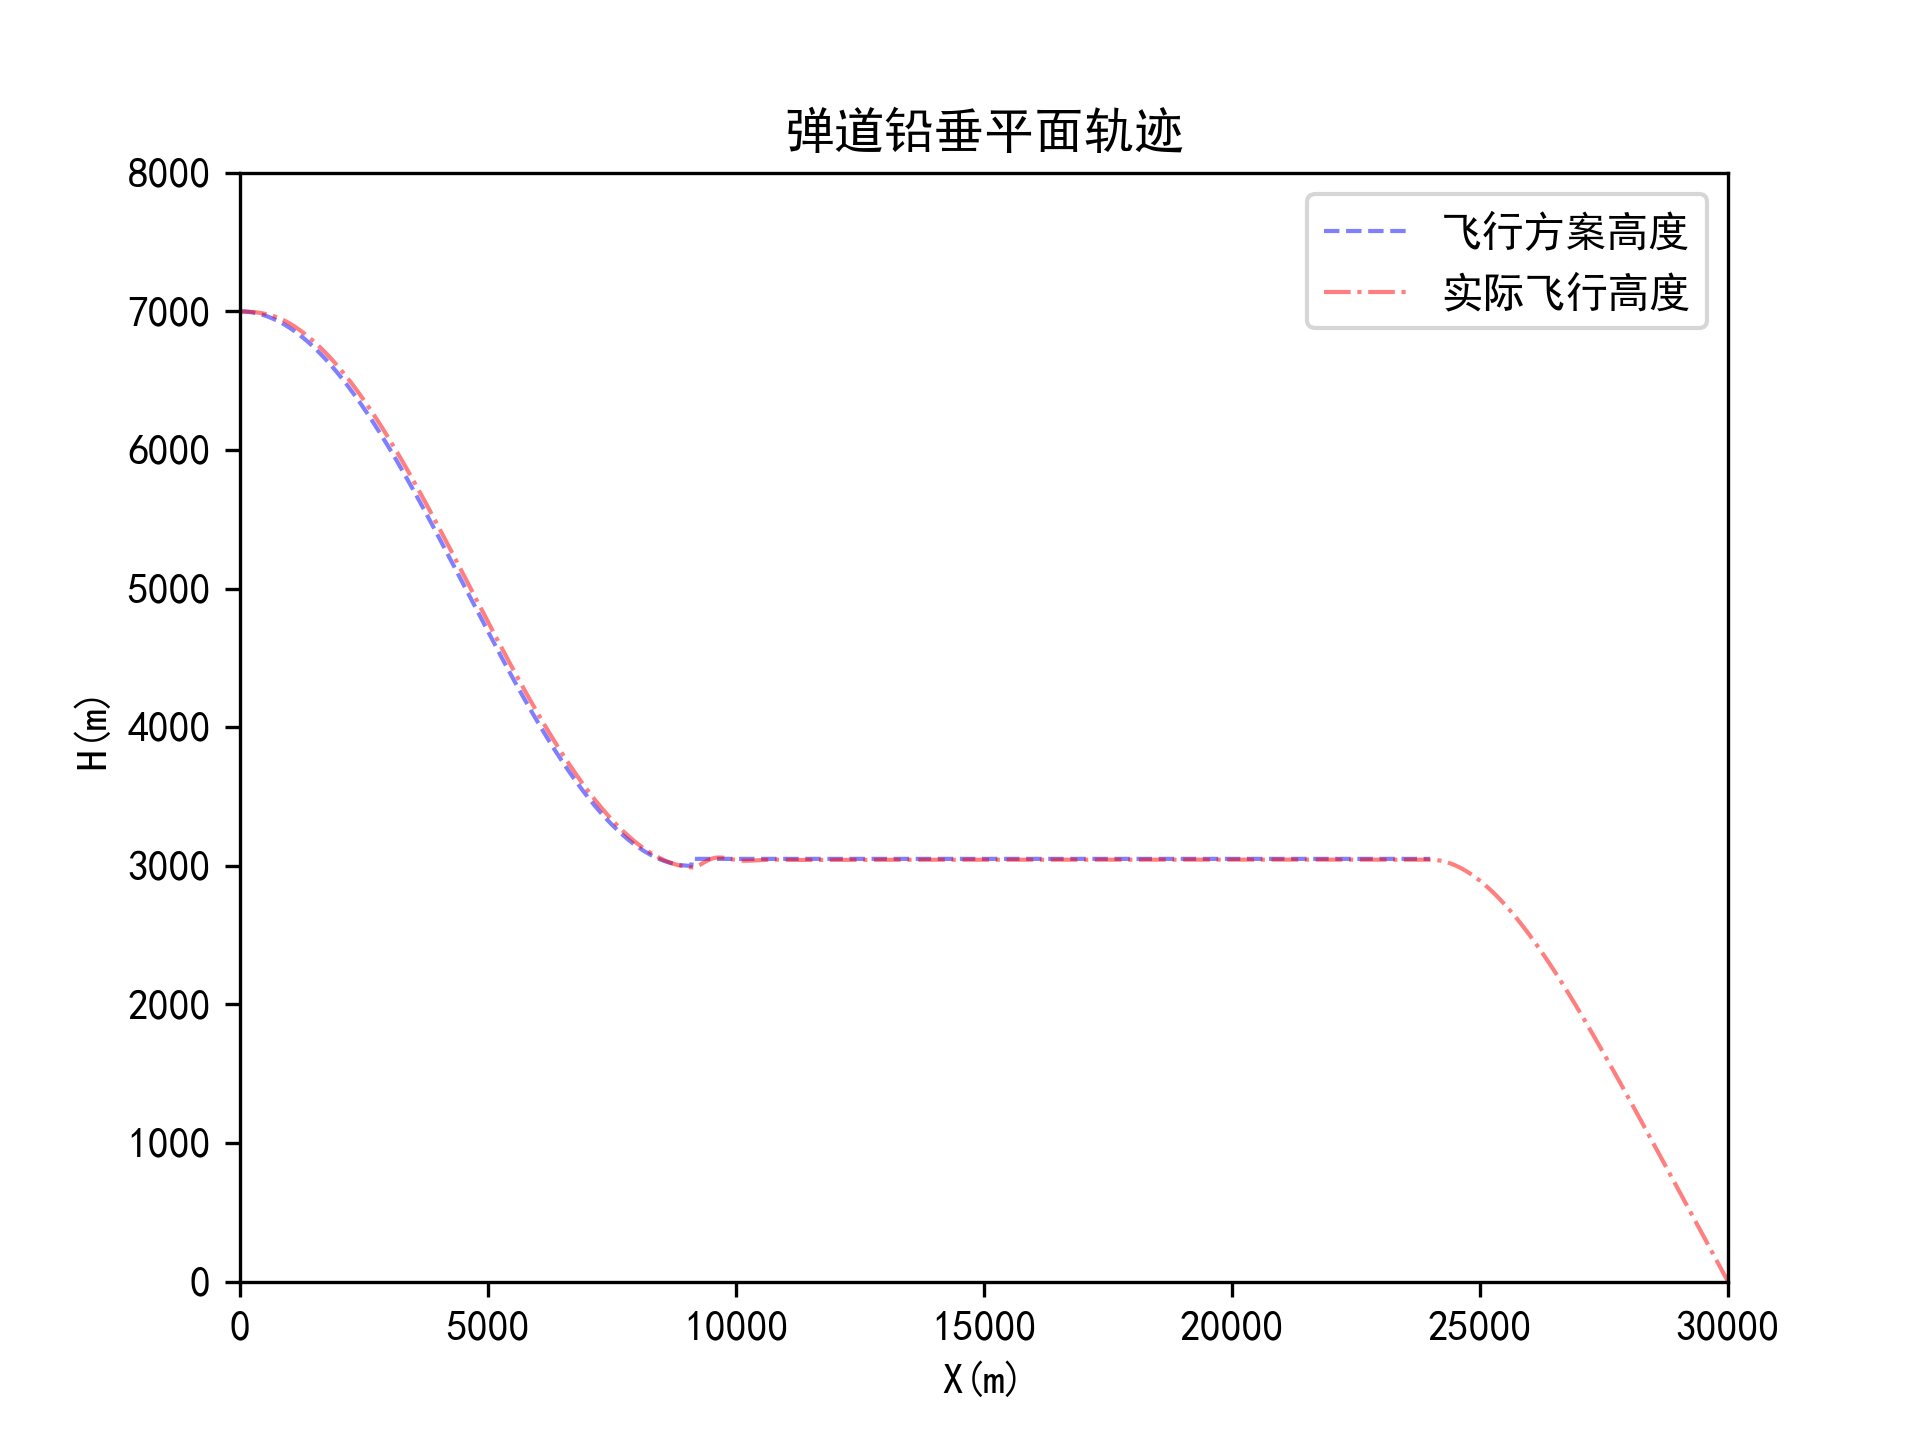
\includegraphics[width=130mm]{img/飞行轨迹.png}
    \caption{导弹飞行轨迹图}
\end{figure}

\begin{figure}[H]
    \centering
    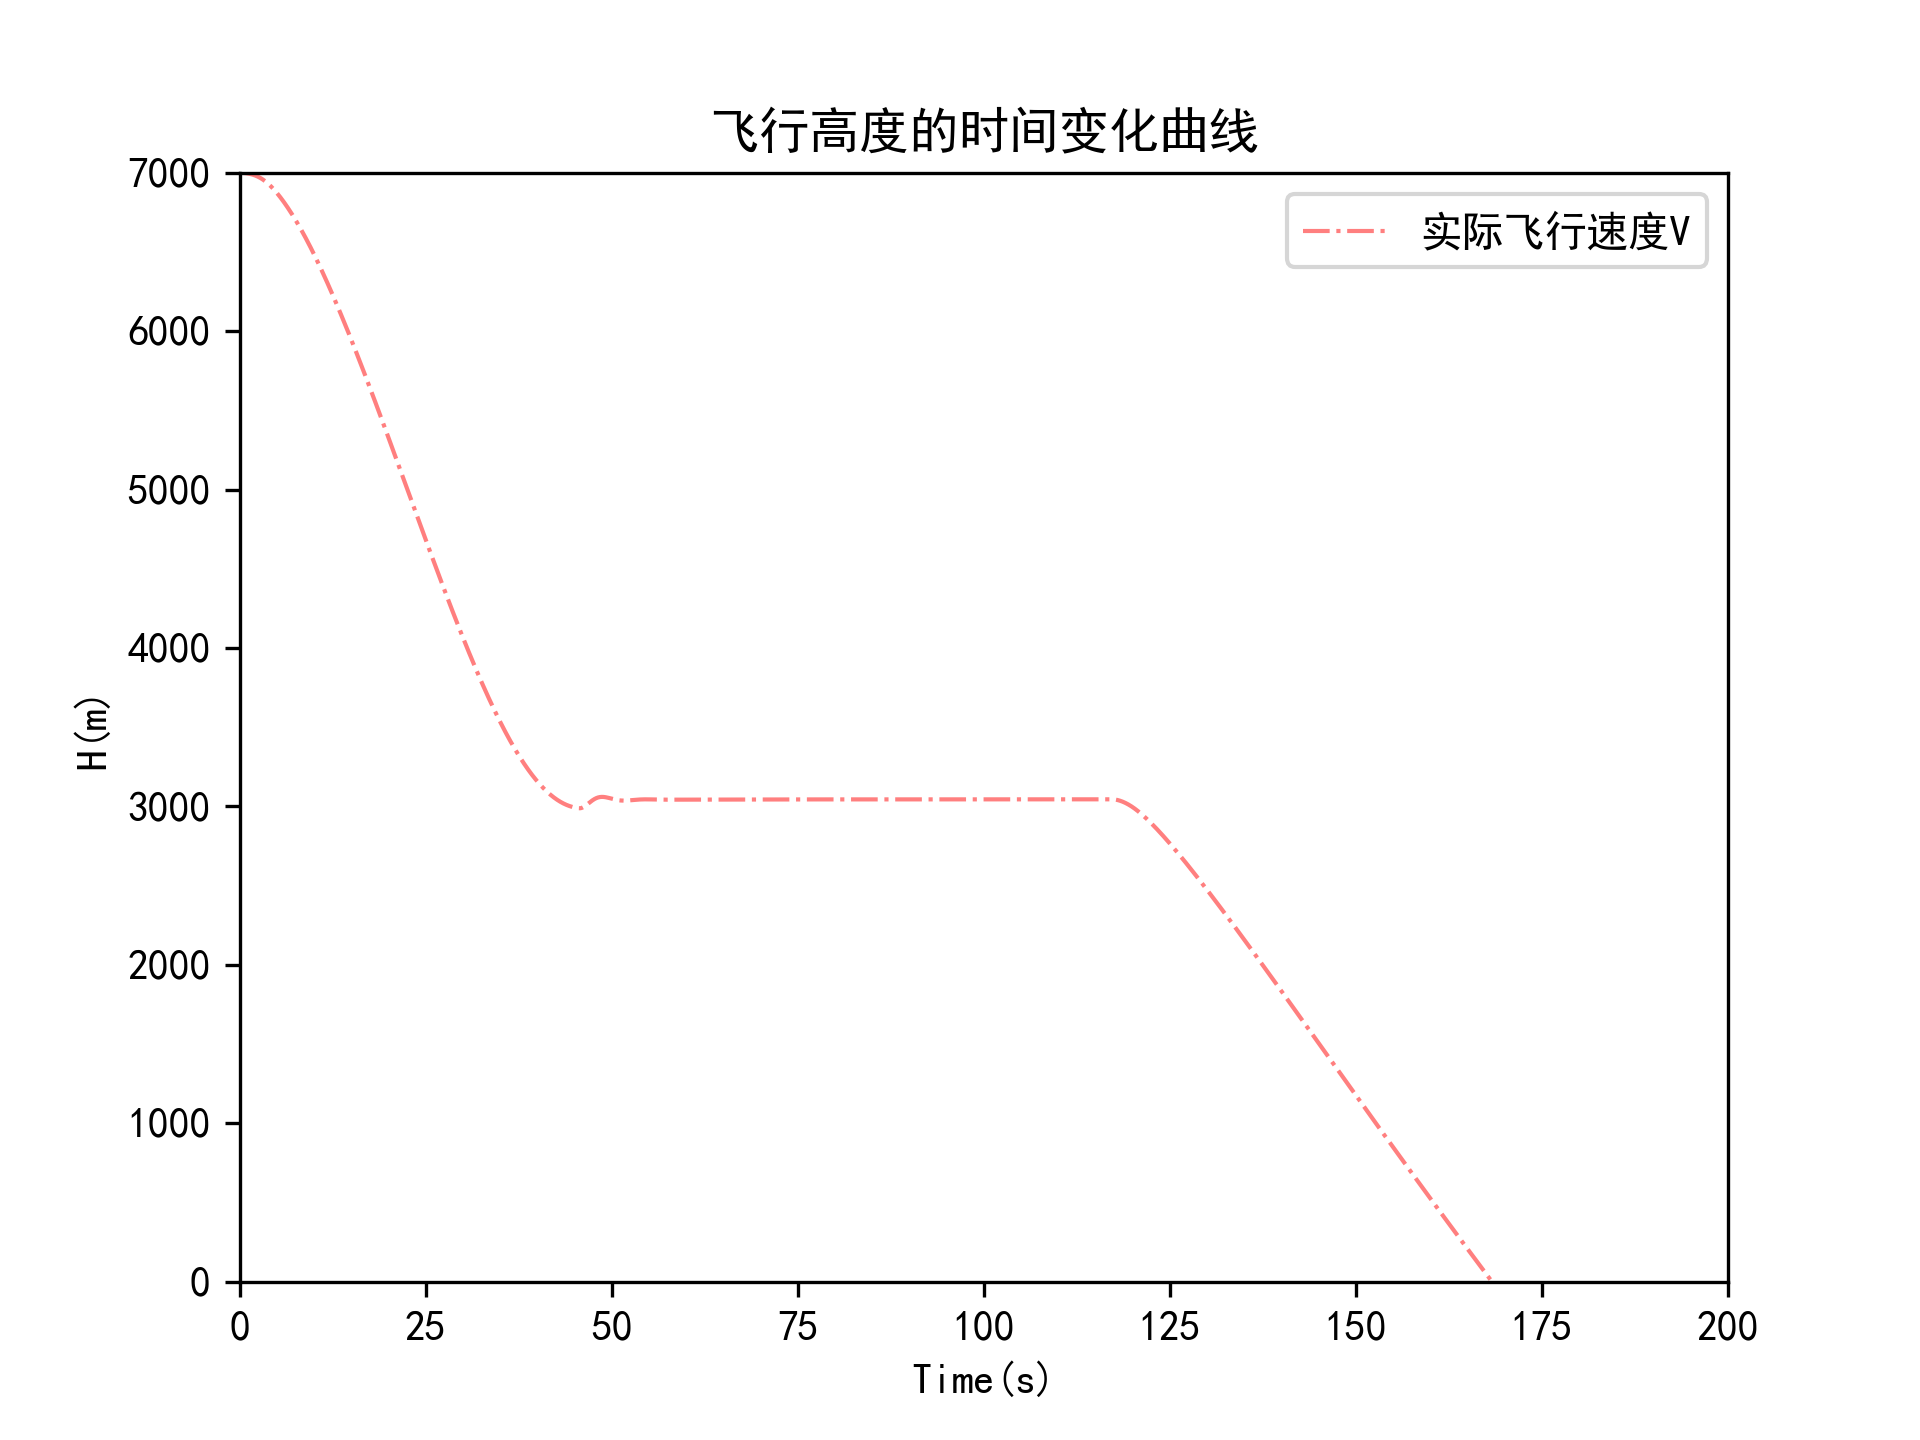
\includegraphics[width=130mm]{img/飞行高度.png}
    \caption{导弹飞行高度的时间曲线图}
\end{figure}
\begin{figure}[H]
    \centering
    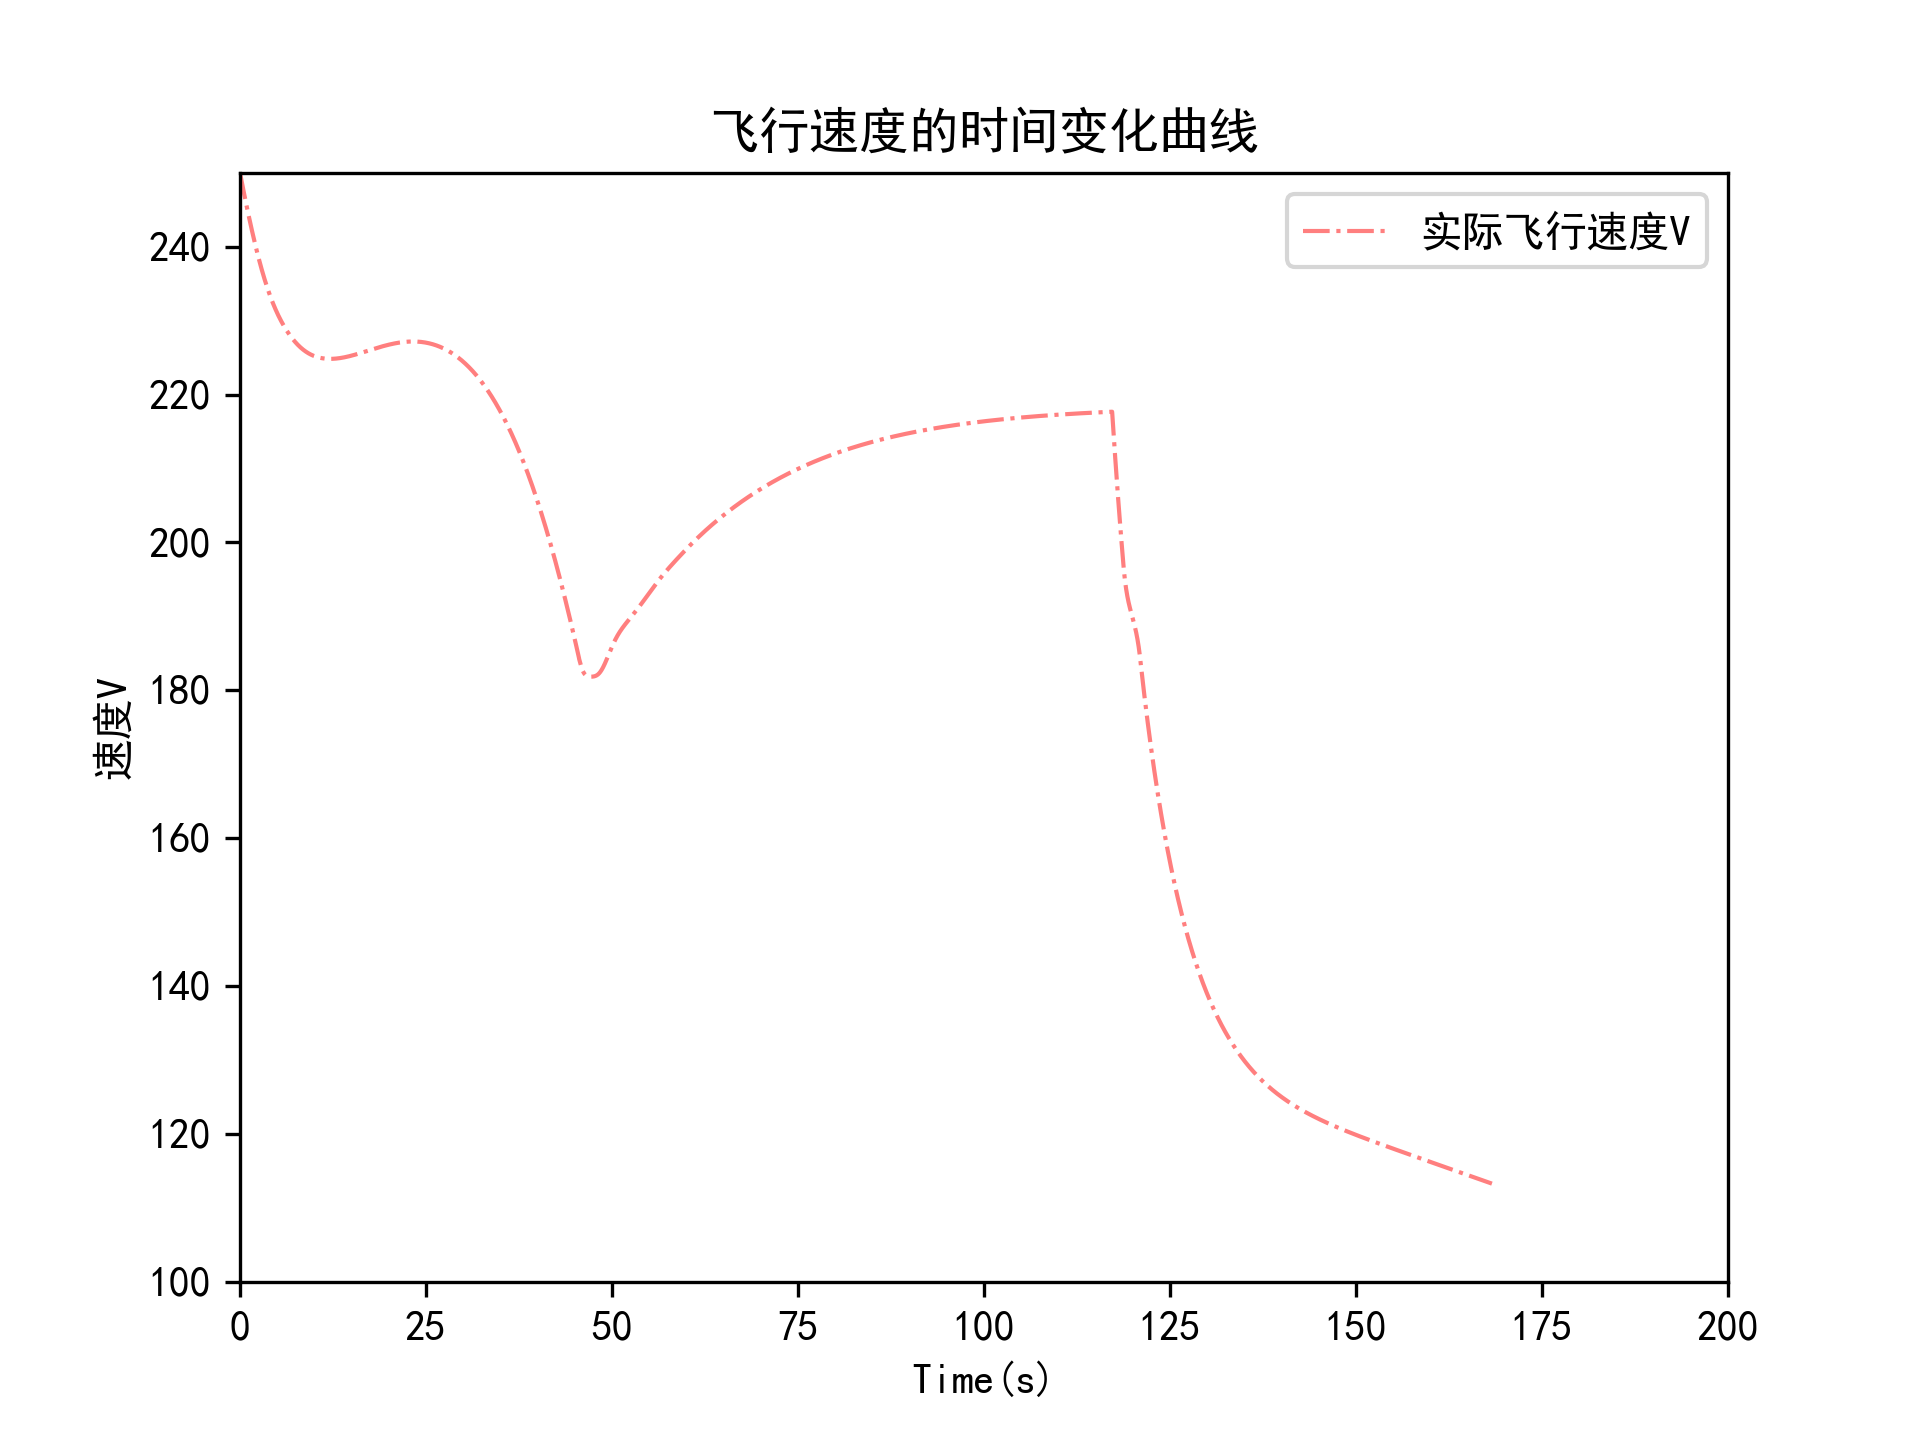
\includegraphics[width=130mm]{img/飞行速度.png}
    \caption{导弹飞行速度的时间曲线图}
\end{figure}
\begin{figure}[H]
    \centering
    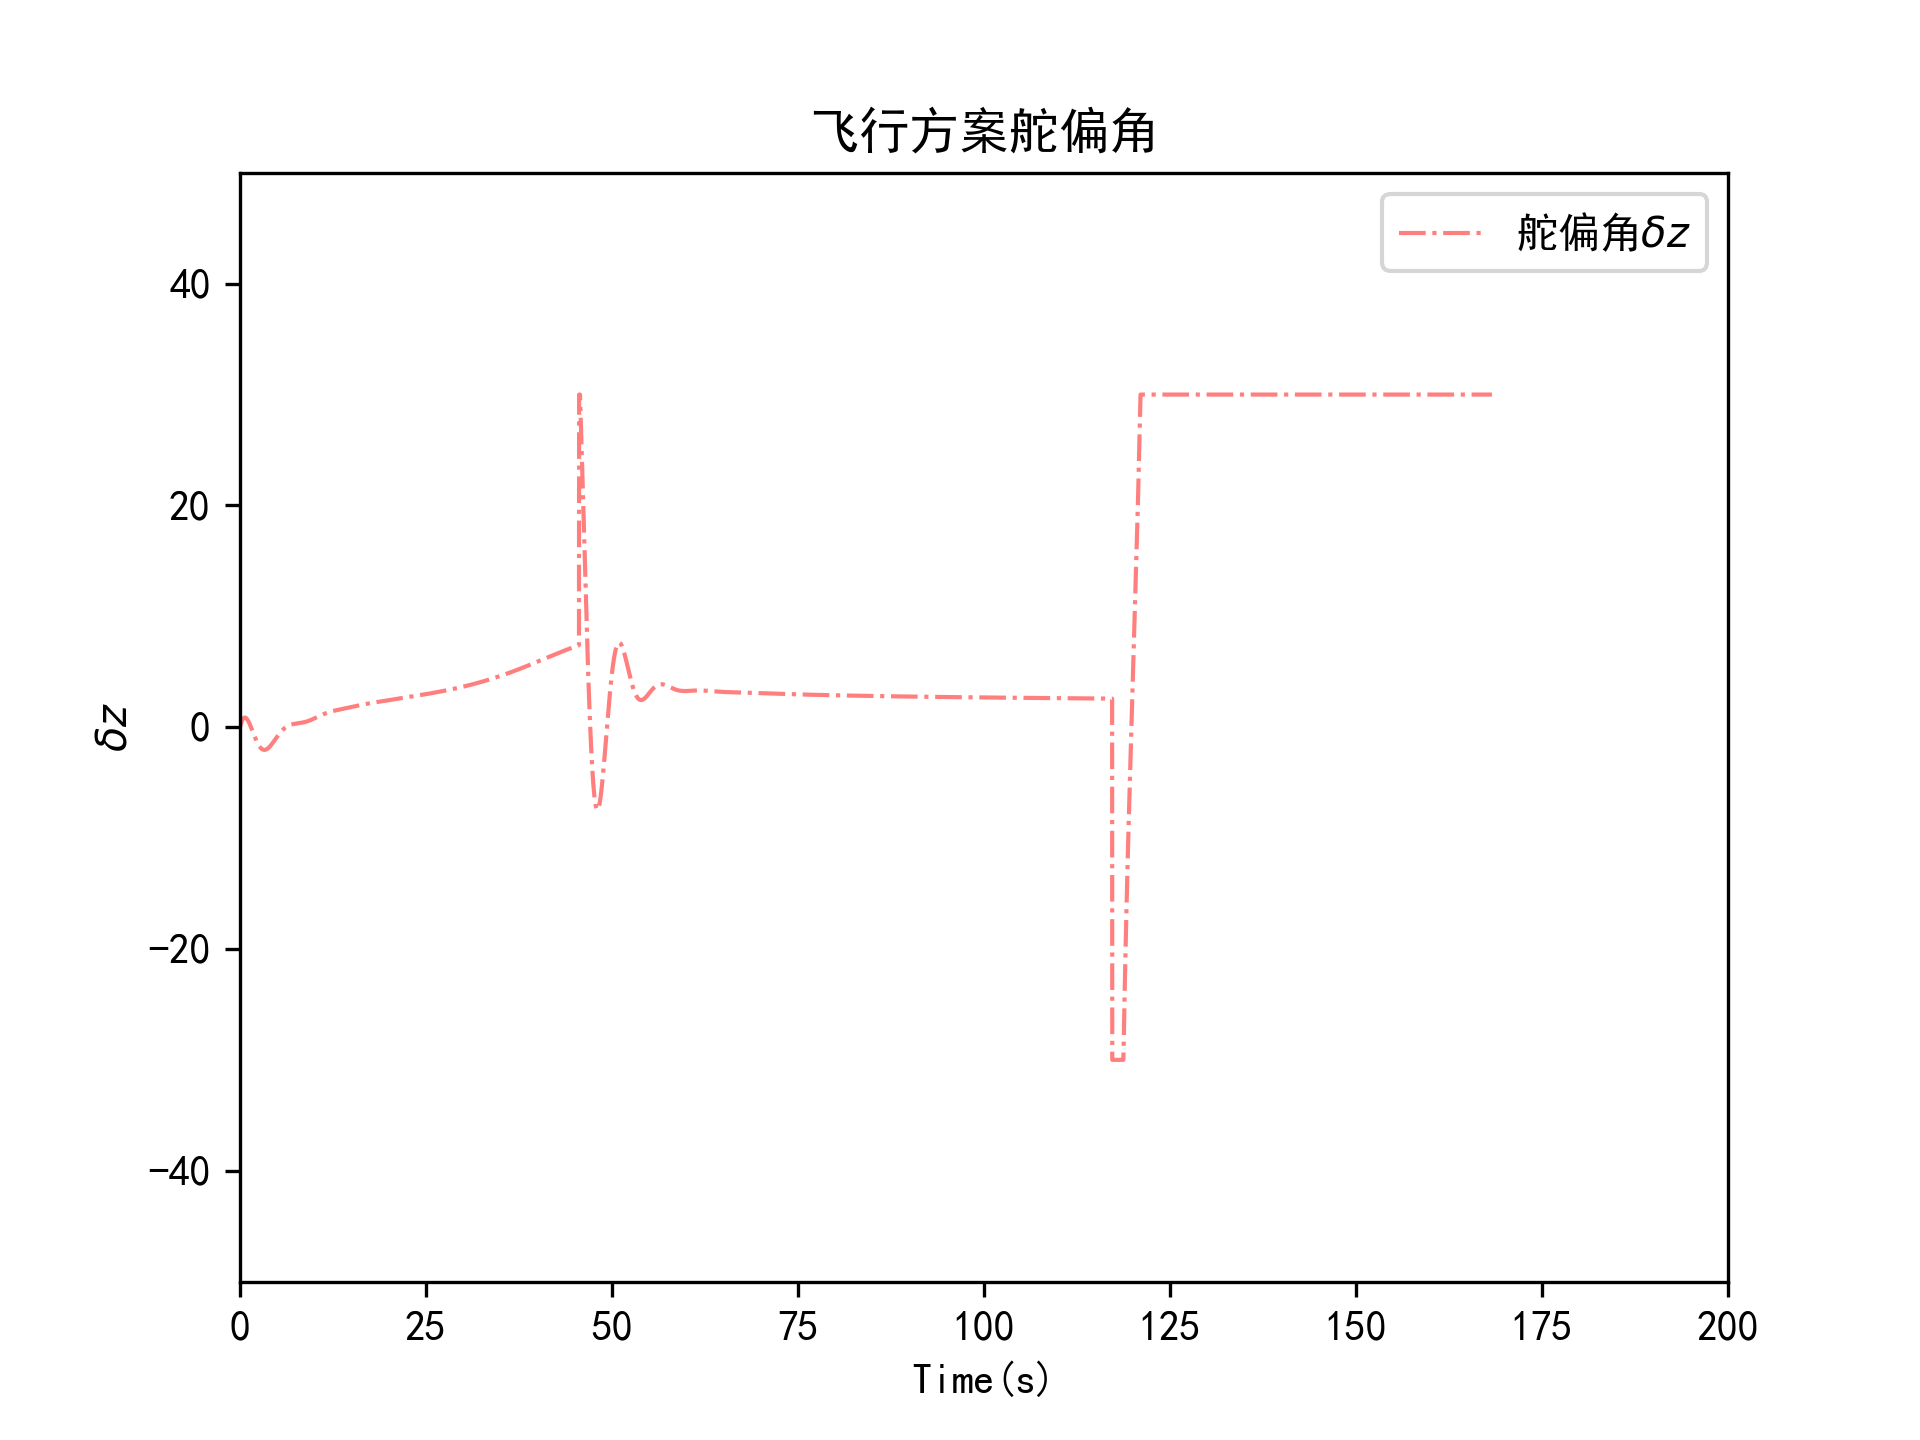
\includegraphics[width=130mm]{img/飞行舵偏角.png}
    \caption{导弹飞行舵偏角的时间曲线图}
\end{figure}
\begin{figure}[H]
    \centering
    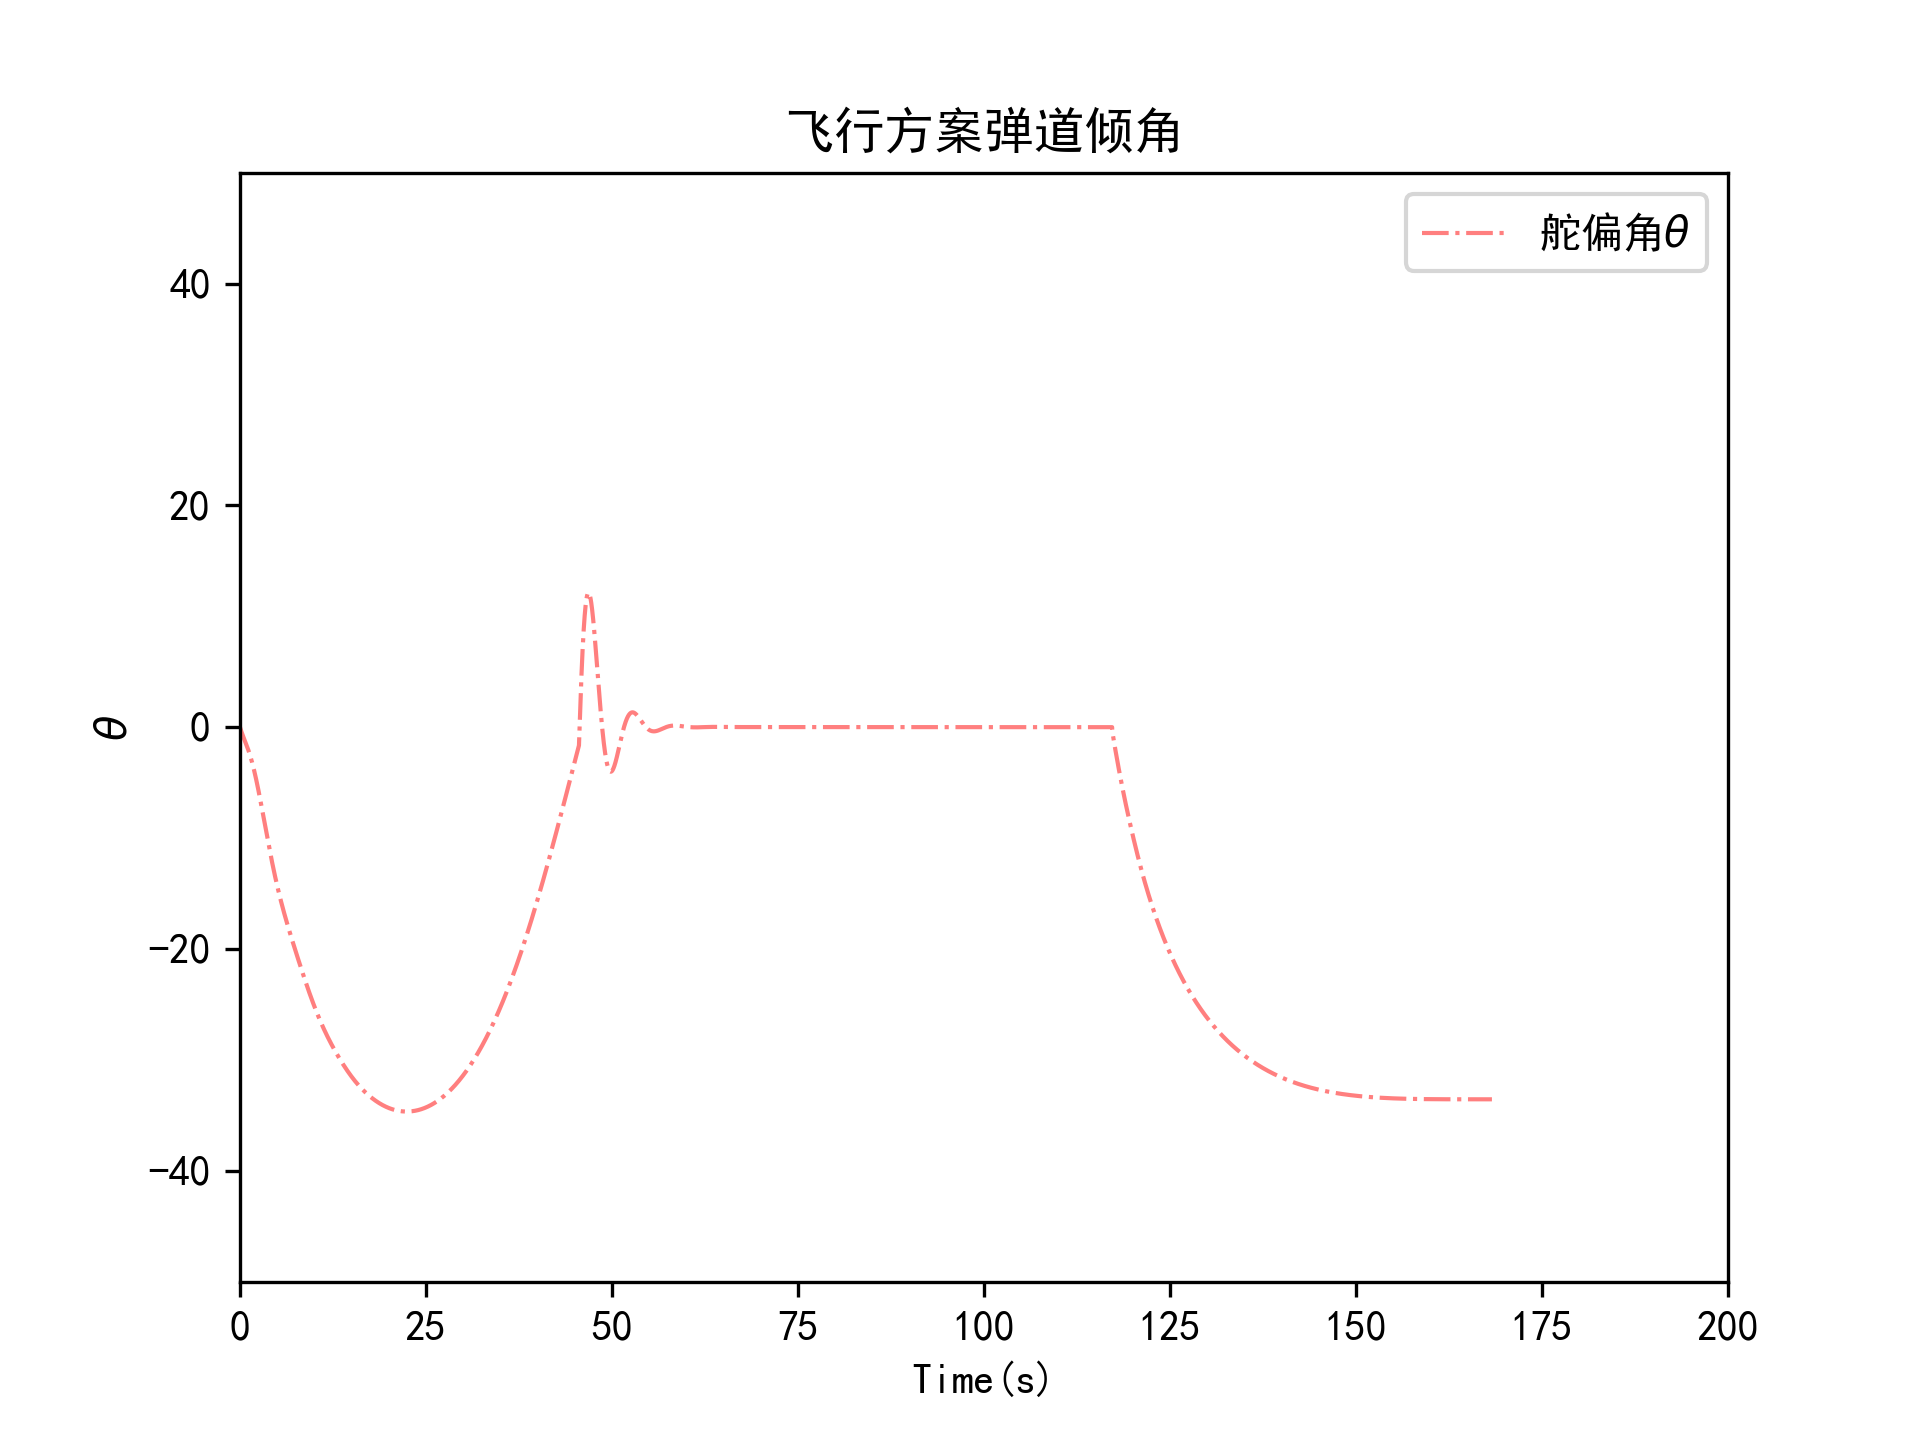
\includegraphics[width=130mm]{img/飞行弹道倾角.png}
    \caption{导弹飞行弹道倾角的时间曲线图}
\end{figure}

\section*{\zihao{-4} 四、结果分析}

\noindent {\heiti 1.$k_{\varphi}$的影响:}
\begin{figure}[H]
    \centering
    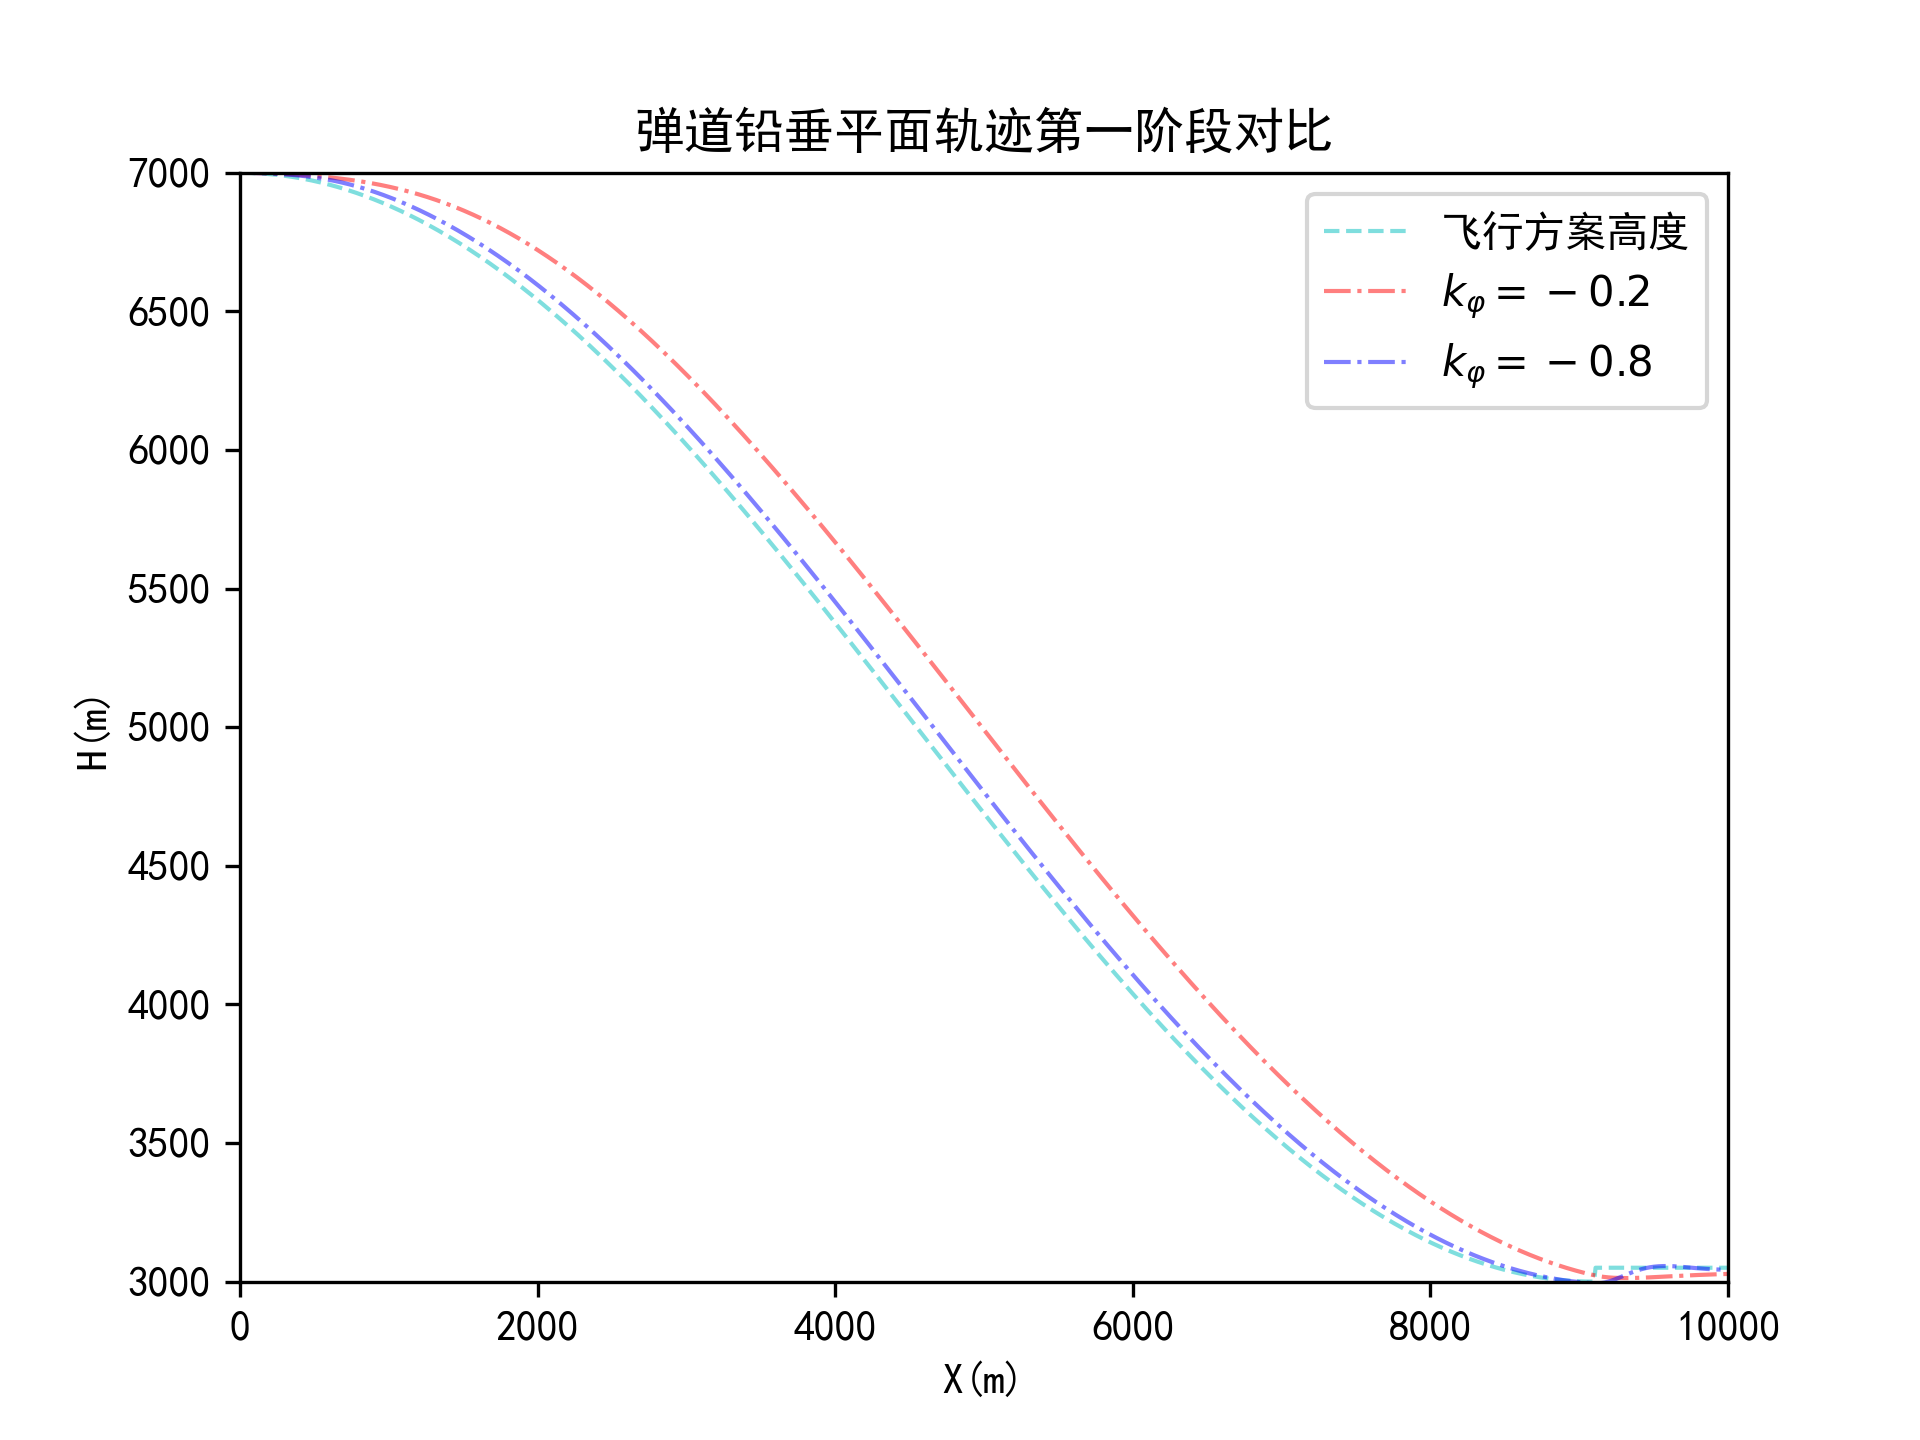
\includegraphics[width=70mm]{img/飞行轨迹2.png}
    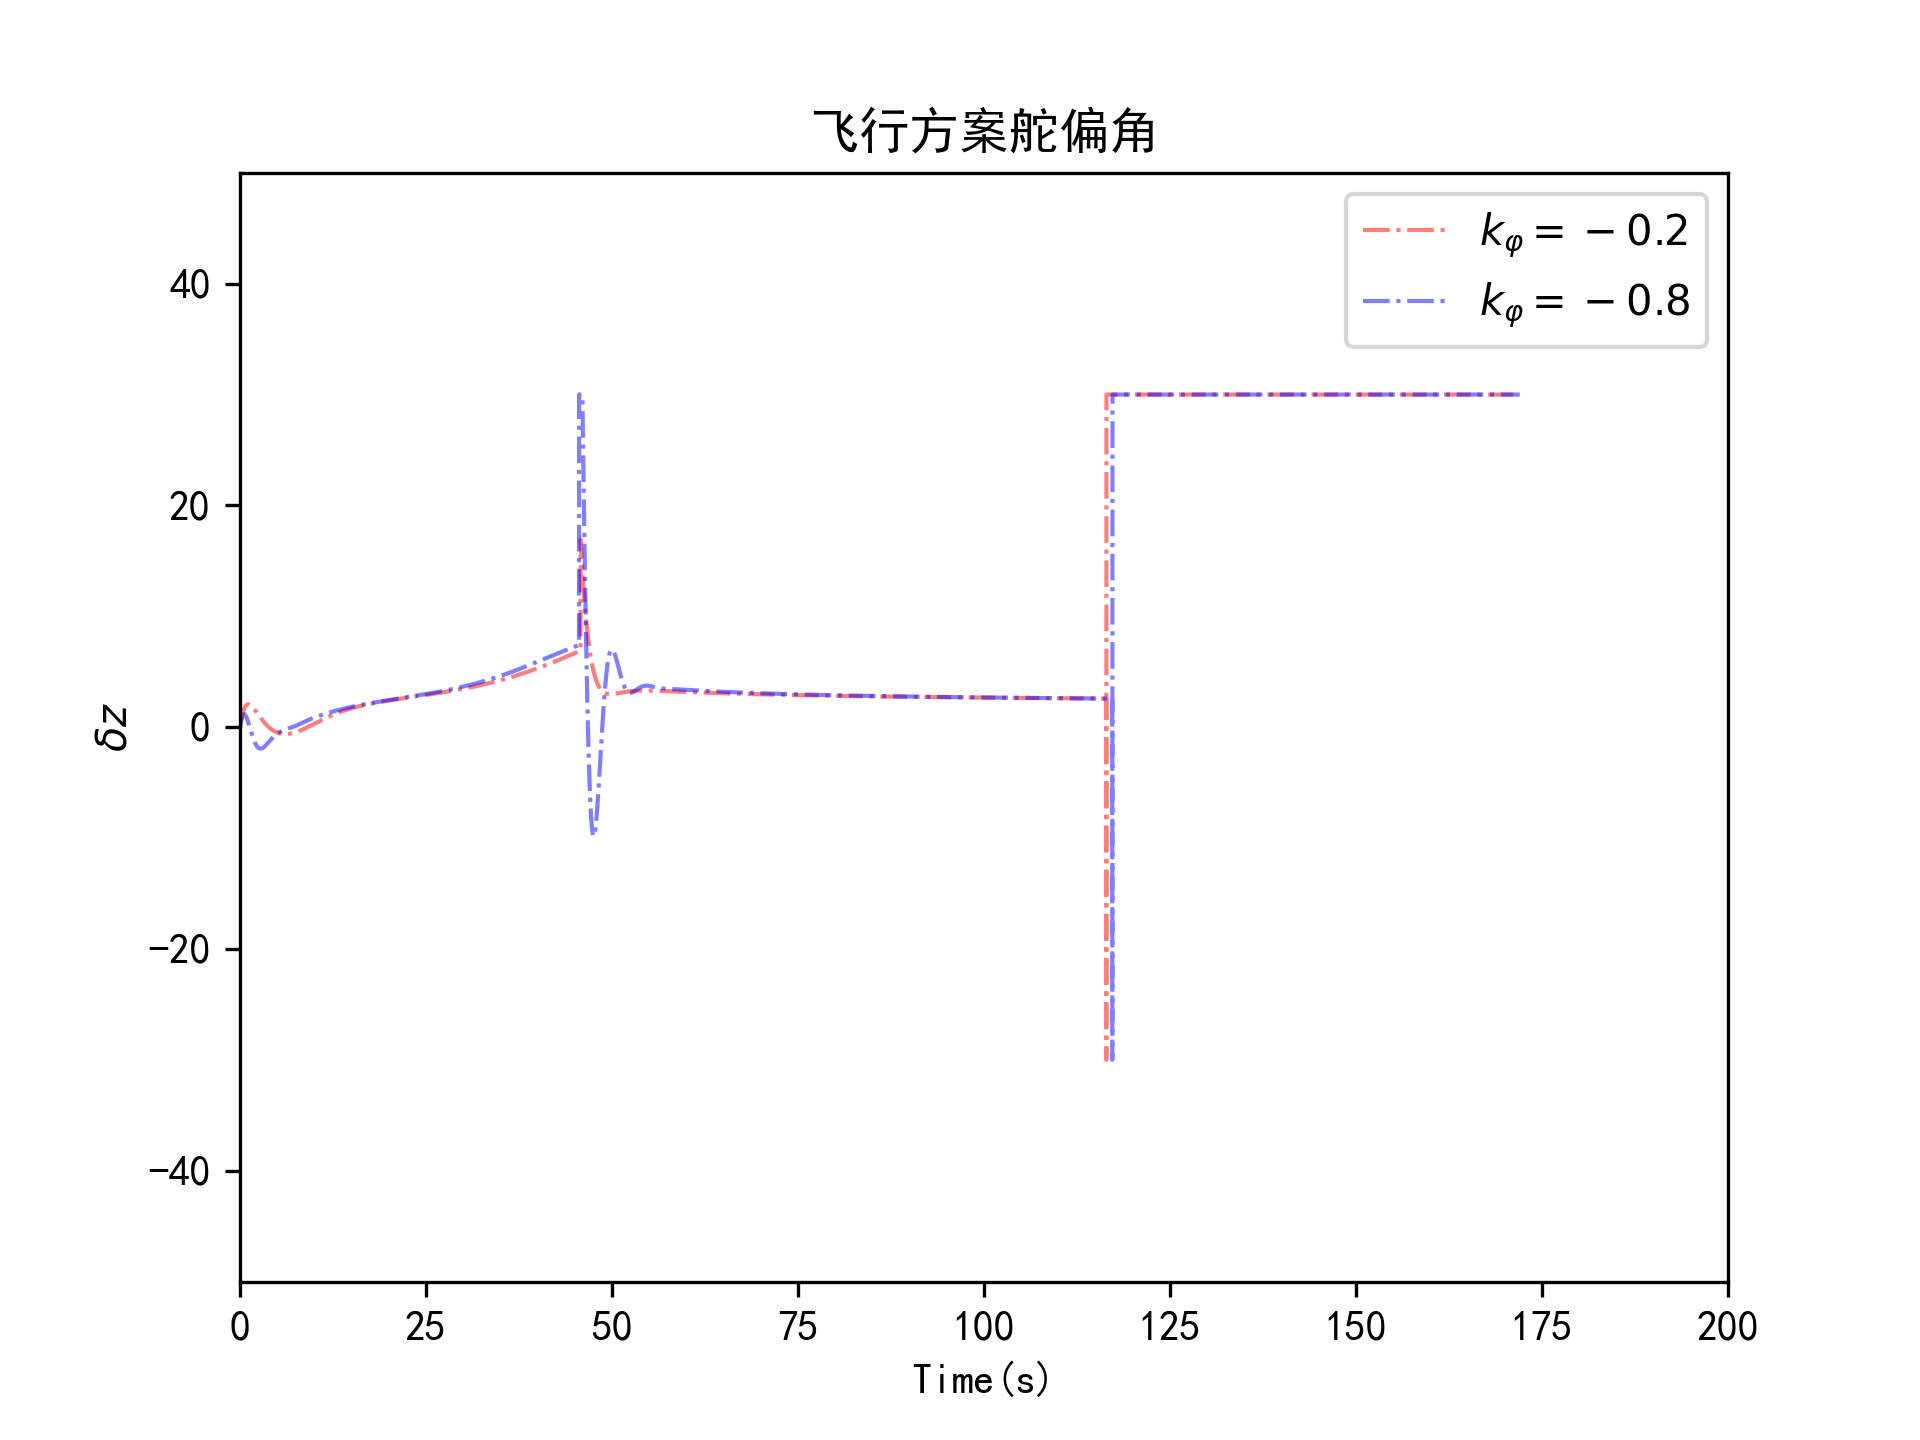
\includegraphics[width=70mm]{img/飞行舵偏角2.png}
    \caption{$K_{\varphi}$大小对导弹飞行弹道和舵偏角的影响}\label{fig:k1}
\end{figure}

如图~\ref{fig:k1}所示,$K_{\varphi}$是理想控制方程的放大系数,$K_{\varphi}$绝对值越大,导弹越快地恢复到预定的飞行方案。

\noindent {\heiti 2.$\dot{K}_{\varphi}$的影响:}
\begin{figure}[H]
    \centering
    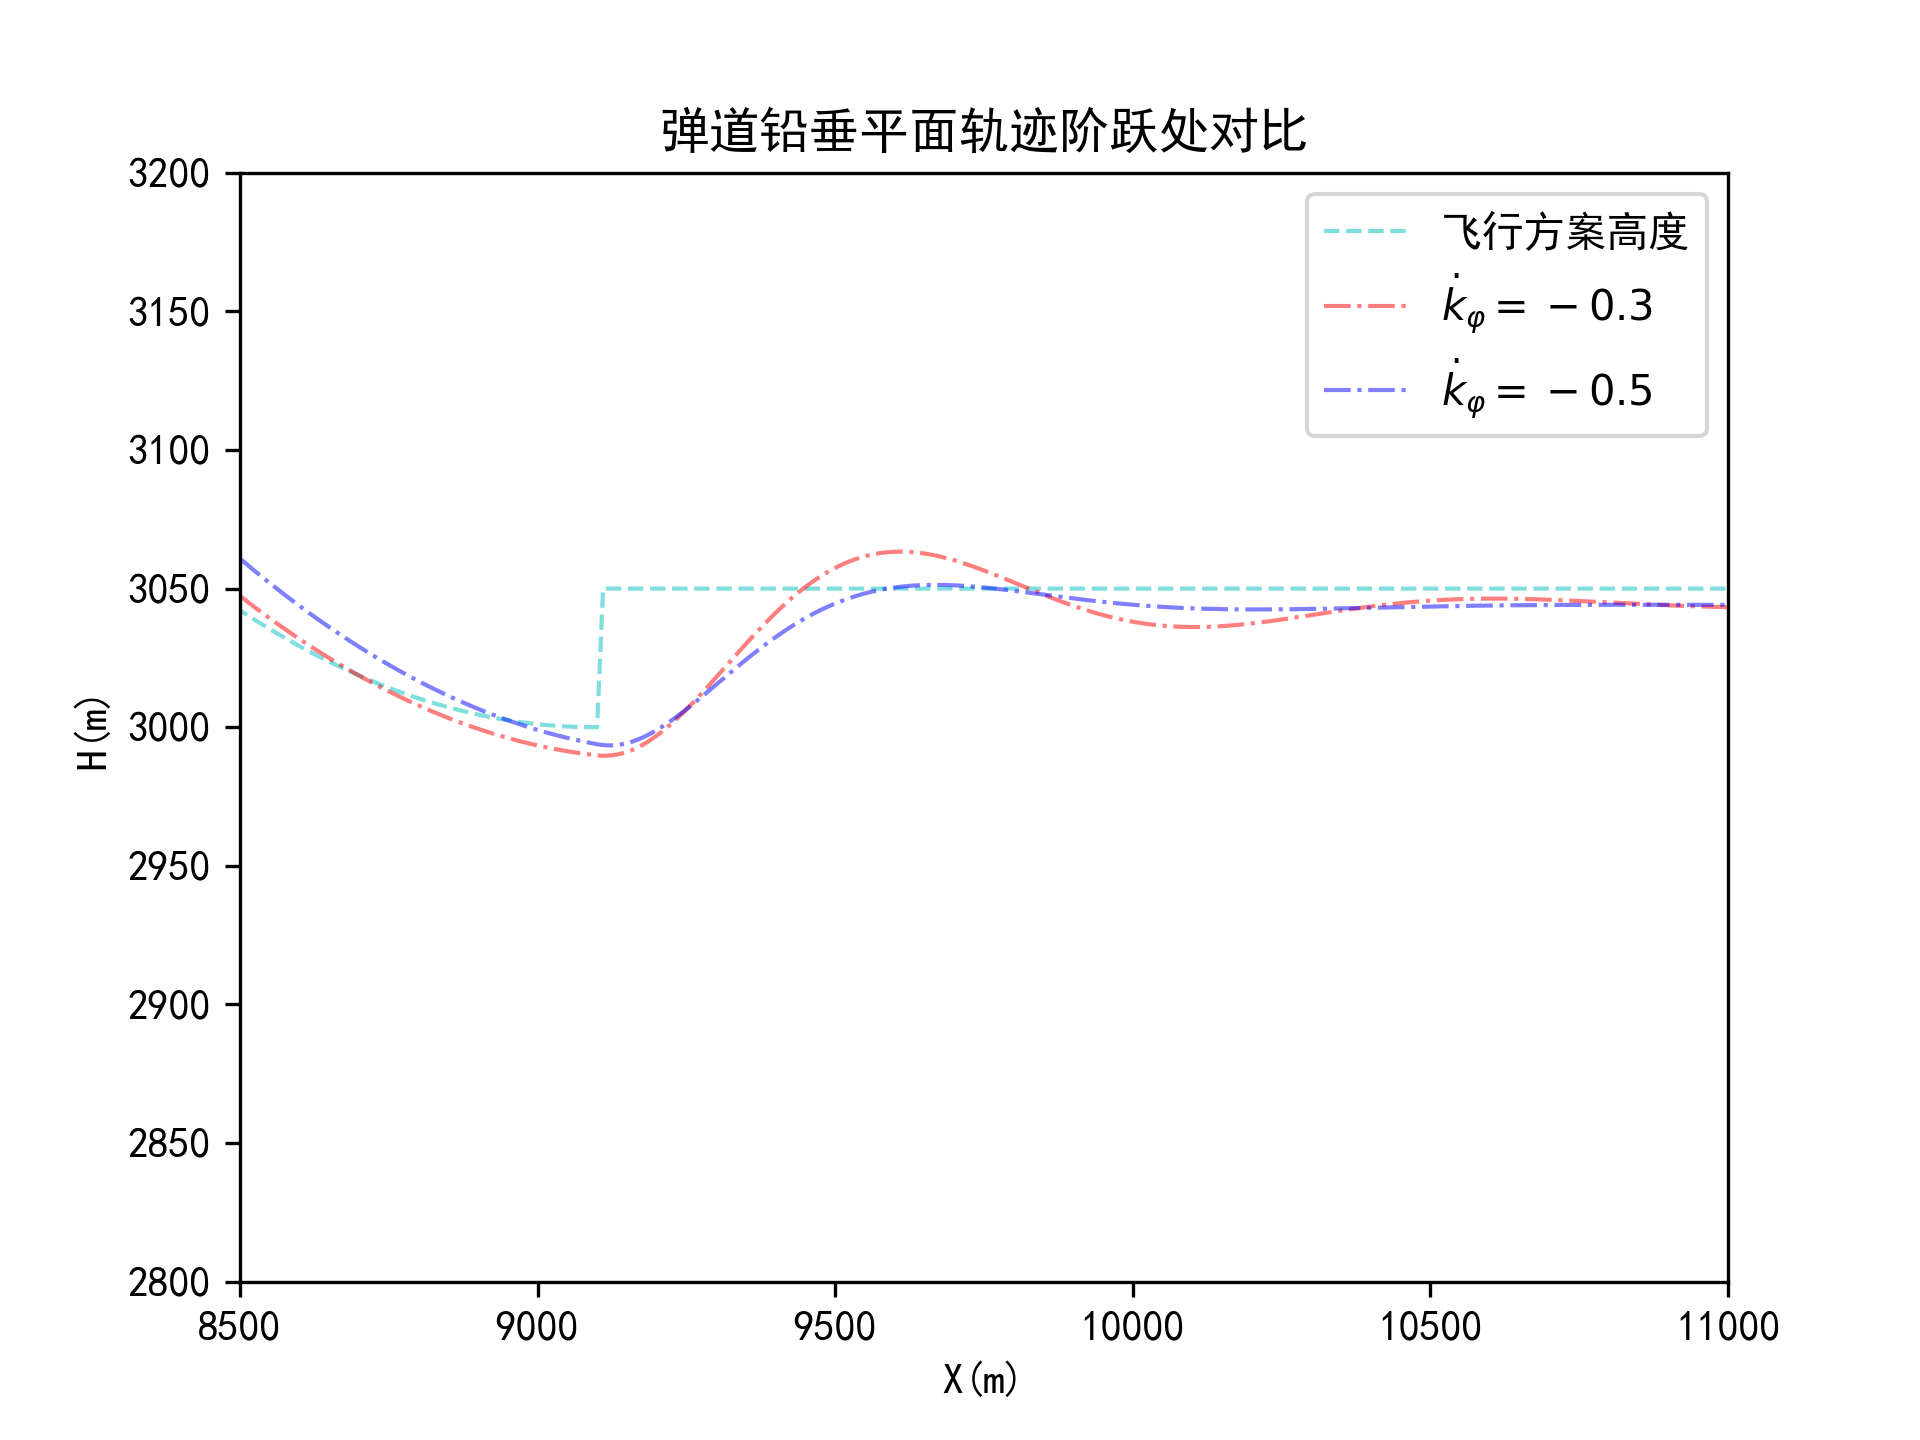
\includegraphics[width=70mm]{img/飞行轨迹3.png}
    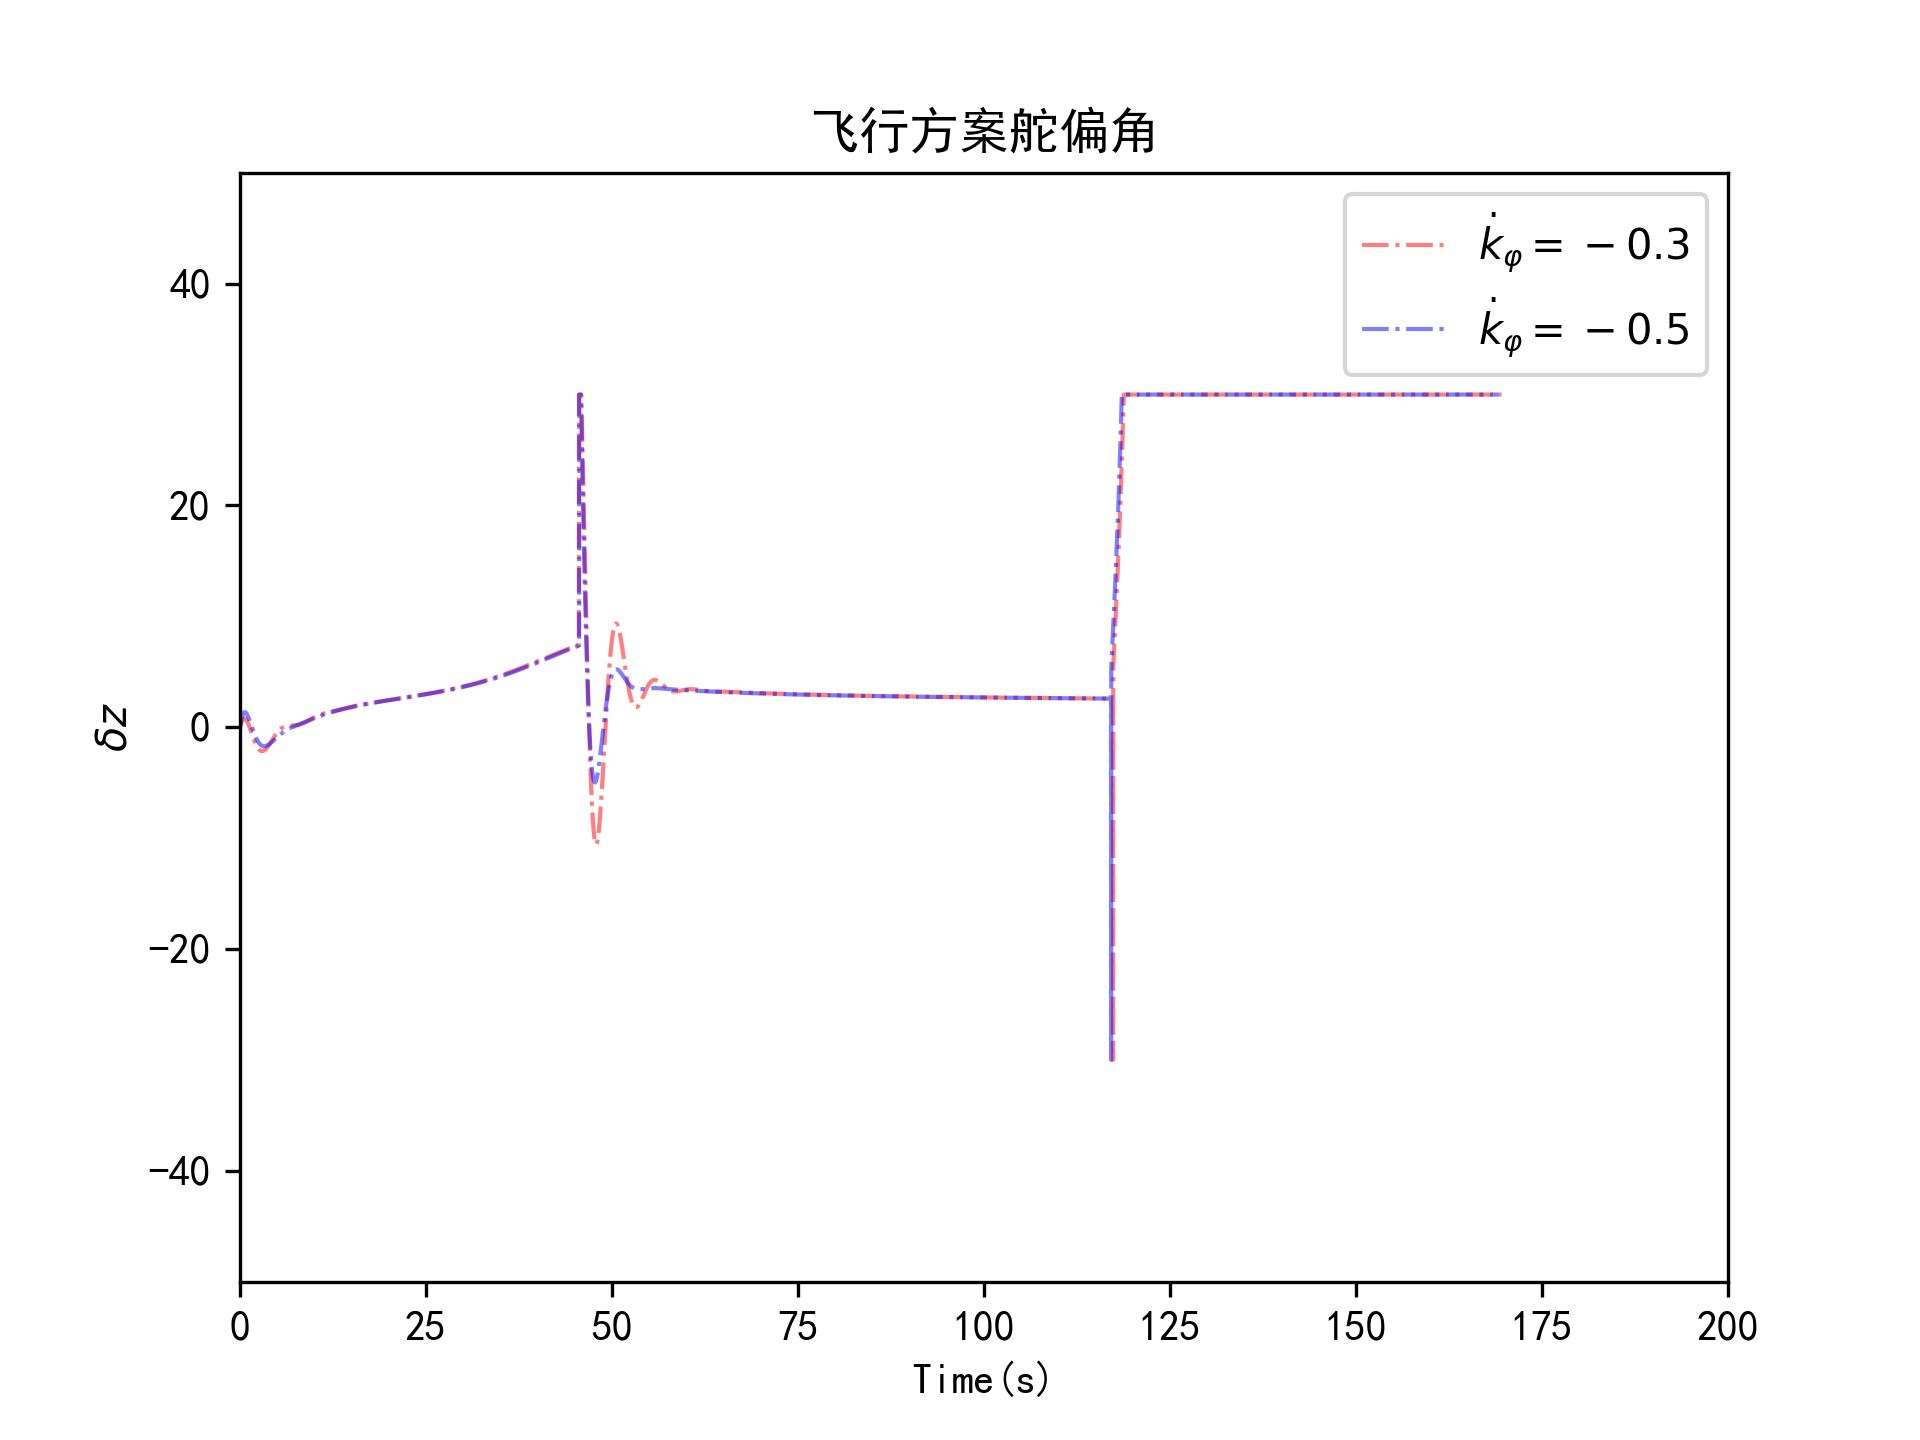
\includegraphics[width=70mm]{img/飞行舵偏角3.png}
    \caption{$\dot{K}_{\varphi}$大小对导弹飞行弹道和舵偏角的影响}\label{fig:k2}
\end{figure}

如图~\ref{fig:k2}所示,$\dot{K}_{\varphi}$是用于减小超调量的放大系数,起到阻尼作用,$k_{\varphi}$绝对值越大,导弹越快地稳定到预定的飞行方案。


\noindent {\heiti 3.${k}_{3}$的影响:}
\begin{figure}[H]
    \centering
    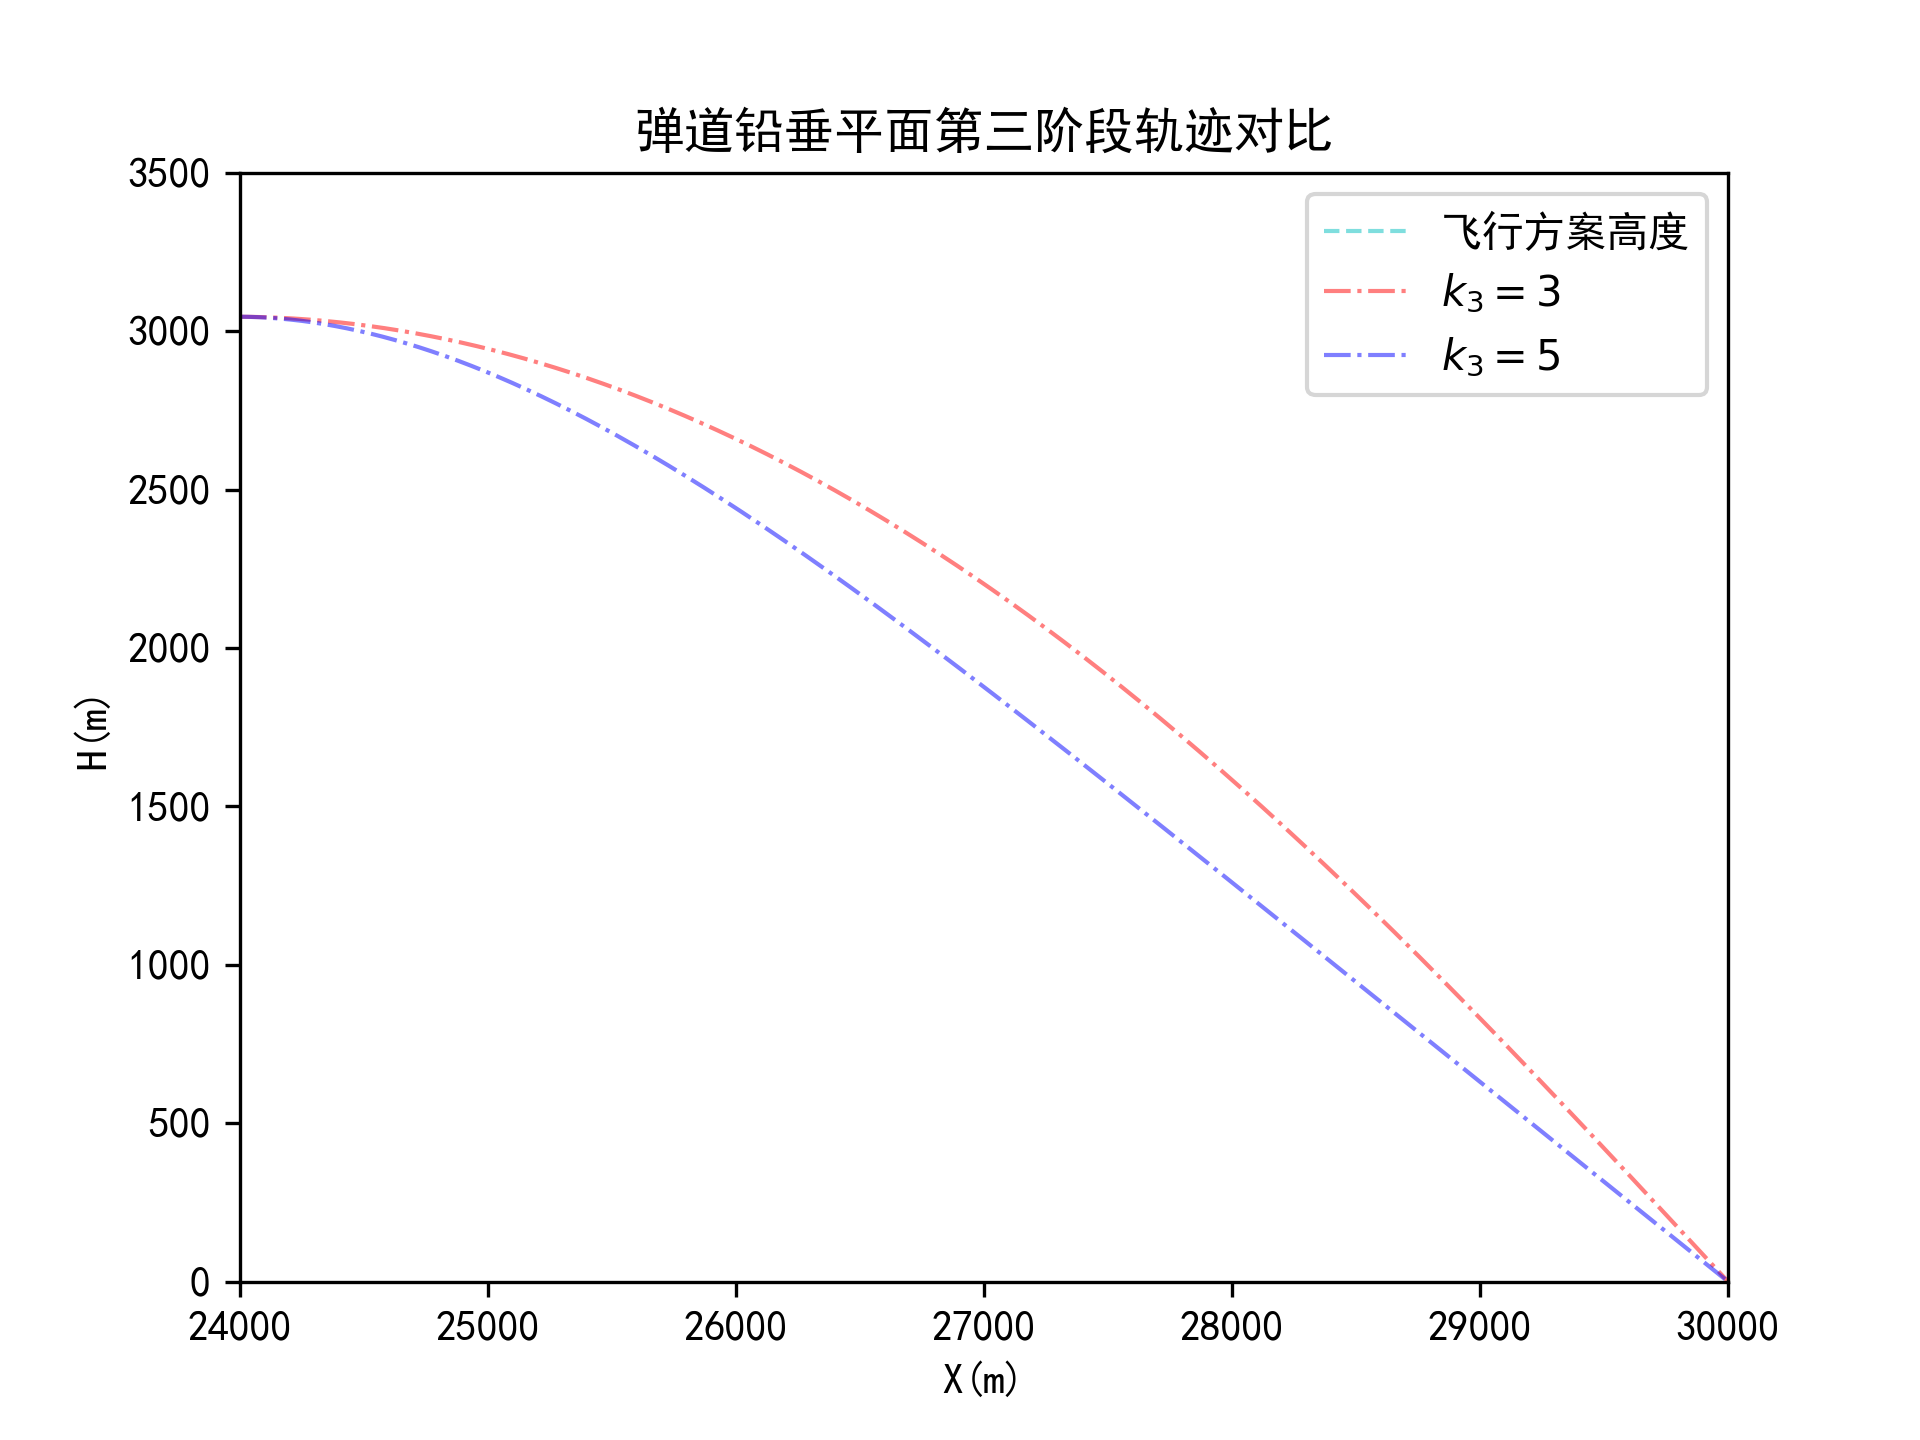
\includegraphics[width=70mm]{img/飞行轨迹4.png}
    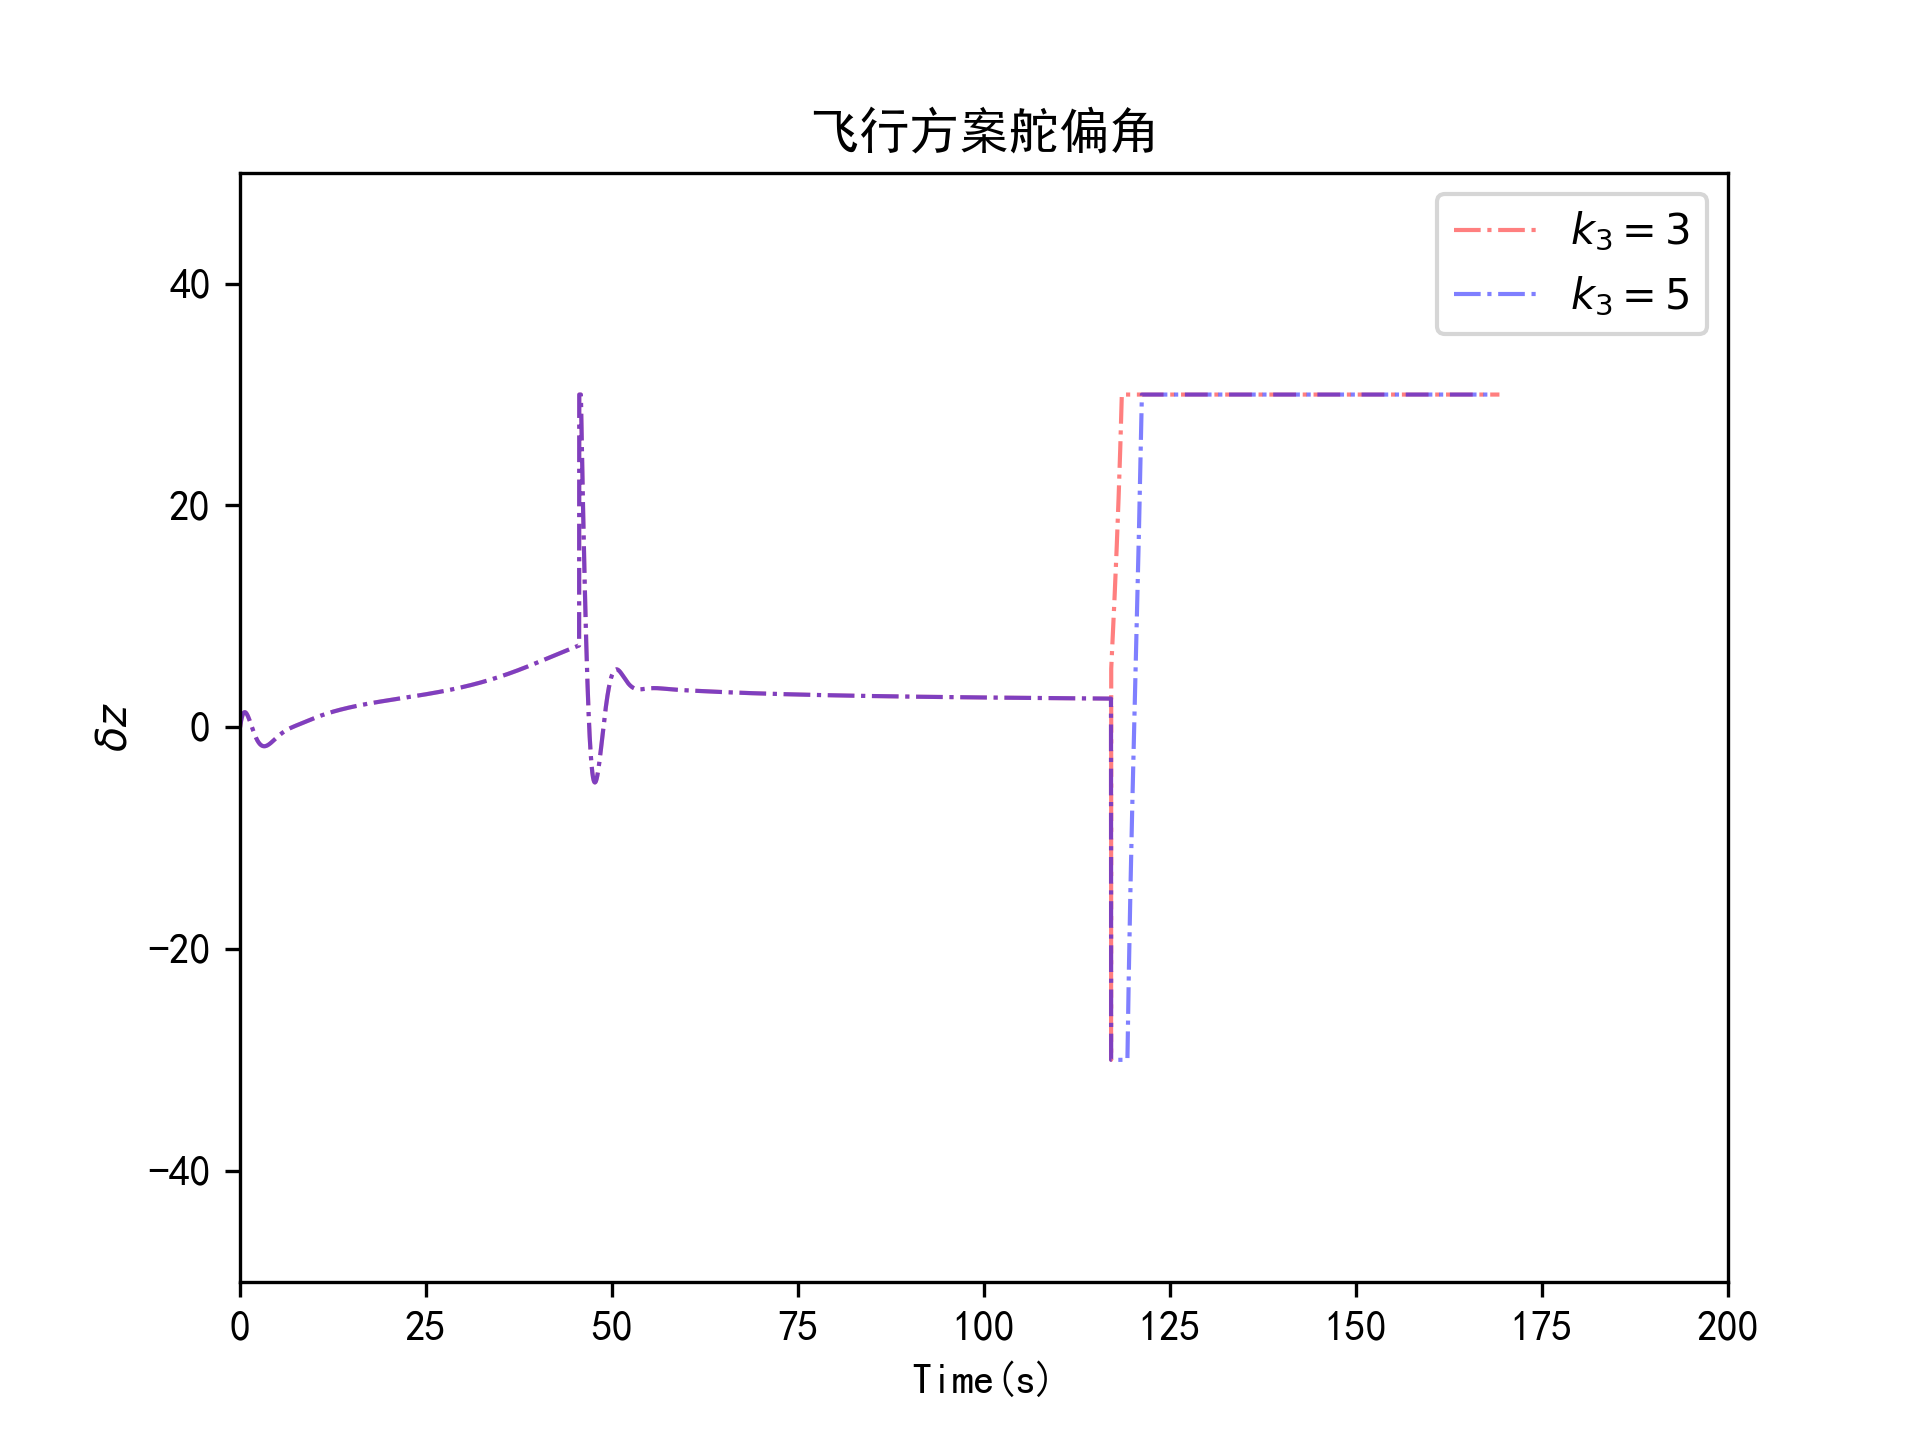
\includegraphics[width=70mm]{img/飞行舵偏角4.png}
    \caption{$k_3$大小对导弹飞行弹道和舵偏角的影响}\label{fig:k3}
\end{figure}
如图~\ref{fig:k3}所示,$K_{3}$是比例导引法的比例系数,$K_3$越大,后期弹道约平直。
~\\
~\\

\bf 注:第三阶段的舵偏角由于使用显式的Euler法计算,结果有一定的发散。
\clearpage
\lstinputlisting[
    style       =   Python,
    caption     =   {\bf main.py},
    label       =   {main.py}
]{./code/main.py}



\clearpage
\lstinputlisting[
    style       =   Python,
    caption     =   {\bf comparis.py},
    label       =   {comparison.py}
]{./code/comparison.py}


\end{document}
